\title{Nonparametric Goodness-of-Fit Tests for Discrete Null Distributions}
\author{by Taylor B. Arnold and John W. Emerson}

\maketitle

\abstract{
A general theory for extending nonparametric goodness-of-fit tests
to discrete null distributions has existed
for several decades. Despite this, modern statistical software
has generally failed to provide this methodology
to users. We offer a revision of R's \code{ks.test()} function
and a new \code{cvm.test()} function that serve to fill this need
in the R language for two of the most popular nonparametric
goodness-of-fit tests. This paper describes these contributions and
provides examples of their usage. Particular attention is given
to various numerical issues that arise in their implementation.
}



\section{Introduction}

%General idea of goodness-of-fit tests (hypothesis test about underlying distribution).
%Given an observed sequence of data, the typical question of statistical inference is to determine
%the underlying process from which it came. 
Goodness-of-fit tests are used to assess whether data are consistent
with a hypothesized null distribution.  The $\chi^2$ test the best-known
parametric goodness-of-fit test, while the most popular nonparametric tests
are the classic test proposed by Kolmogorov and Smirnov followed closely by
several variants on an estimation procedure proposed by
Cram\'{e}r and von Mises (tests sometimes called Cram\'{e}r-von Mises-Smirnov
tests, or simply Cram\'{e}r-von Mises tests).

In their most basic form, the nonparametric goodness-of-fit
tests are intended for continuous null distributions, but they have
also been adapted for use with discrete null distributions.  Unfortunately,
most modern statistical software has failed to incorporate these discrete
versions, leaving researchers with the $\chi^2$ test or in the unfortunate
position of applying a nonparametric test designed for continuous null
distributions and hoping for the best.
As we will see, the latter choice can be particularly dangerous
in the small sample setting. This paper presents a revision of R's
\code{ks.test()} function and a new \code{cvm.test()} function to
fill this void for researchers and practitioners in the R environment. 

%Given a particular null distribution, goodness-of-fit tests 
%are used in order to test whether it is likely that the data were
%generated via the null distribution.

%Why we use non-parametric tests (power to interesting shifts; robustness to underlying assumptions).
%While almost any hypothesis test can be viewed as a variant on a
%goodness-of-fit test, the term ``goodness-of-fit test'' is typically
%reserved for those tests which are nonparametric in nature. 
%That is, they do not conduct the hypothesis testing 
%through the explicit calculation of the parameters generating the data. Instead, they %generally attempt to
%calculate differences between the empirical distribution of the observed data and the overall distribution 
%of the null model. In many cases these tests are preferential since they tend to have an increased power for 
%interesting deviations from the null model, in exchange for failing to detect less interesting deviations due to 
%factors such as measurement error. By far the most popular of these nonparametric tests are due to Kolmogorov and 
%Smirnov, followed closely by several variants on an estimation procedure proposed by Cram\'{e}r and von Mises. 

% Discrete versions exist; just no code
%While the original aim of nonparametric goodness of fit tests was meant for continuous null distributions, discrete versions
%have existed since the early 1970s. Unfortunately, current statistical software has largely failed to incorporate them.
%This has left the end-user to either use only parametric tests, such as Pearson's Chi-Squared test, or to incorrectly
%apply the functions meant for continuous distributions. 

\section{Kolmogorov-Smirnov Test}

% Most popular choice of test; explain the basic algorithm and purpose for continuous distributions (maybe a few P's).

\subsection{Overview}

Of all the methods for nonparametric goodness-of-fit tests, the most popular is the method devised by Kolmogorov and Smirnov.
It is the only such test built into the base of R. The idea behind it is fairly simple. Given the cumulative distribution
function $F_0(x)$ of the continuous null distribution, and the empirical distribution function $F_{data}(x)$ of the observed data, 
one constructs the statistic:
\begin{align}
D = \sup_x \left| F_0(x)- F_{data}(x) \right|
\end{align}
The distribution of $D$ under the null model does not depend on which null distribution is being used, making this a computationally
attractive method. For a standard treatment of the test and its performance relative to other algorithms see \cite{slakter65}. Two common
alternatives of the above test statistic exist. The absolute value is discarded and the rest is either left alone (the `greater' testing 
alternative) or the supremum is replaced with a negative infimum (the `lesser' hypothesis alternative). These can be helpful depending 
on the nature of the alternative hypotheses for which the test is desired to be powerful towards.

The extension of this result to non-continuous null distributions does not have such a clean solution. The formula of
the test statistic $D$ remains unchanged, however the distribution of the testing statistic is much more difficult. Unlike in the 
continuous case, it ultimately depends on which null model was chosen; this makes it impossible to simply read p-values directly 
off of a fixed table. It was known since at least the 1950's that using the tables for continuous distributions resulted in 
conservative p-values; it was not until \citet{Conover1972} that a method for computing exact p-values in this case was developed.

\subsection{Implementation}

The implementation of the discrete Kolmogorov-Smirnov function consists of two parts. First the particular test statistic needs to be calculated,
and then the p-value for that particular statistic must be computed. 

Given that the test statistic is, theoretically, the same as in the
continuous case it would seem that the first part could be directly taken from the existing procedures. This is, unfortunately, often not the case.
Consider two non-decreasing functions $f$ and $g$, where the function $f$ is a step function with jumps on the set $\{x_1, \ldots x_N \}$ and $g$
is continuous. If we want to determine the supremum of the difference between these two functions notice that:

\begin{align}
\sup_x &\left| f(x)- g(x) \right|   \\
       &= \max_i \left( \left|g(x_i) - f(x_i) \right|, \lim_{x \rightarrow x_i} \left| g(x) - f(x_{i-1}) \right| \right) \\
&=  \max_i \bigg( \left|g(x_i) - f(x_i) \right|, \left| g(x_i) - f(x_{i-1}) \right| \bigg)
\end{align}

Computing the maximum over these $2N$ values (with $f$ equal to $F_{data}(x)$ and $g$ equal to $F_0(x)$ as defined above) is clearly the 
most efficient way to compute the Kolmogorov-Smirnov test statistic when given a continuous null distribution. When the function $g$ is not
continuous, notice that this formula no longer works since in general we cannot replace the limit of $g$ with its value at $x_i$. If it is known that $g$
is also a step function, we could replace the formula for some small $\epsilon$ by:
\begin{align}
\sup_x &\left| f(x)- g(x) \right| =   \\
        &                    \max_i \{ \left|g(x_i) - f(x_i) \right|, \left| g(x_i - \epsilon) - f(x_{i-1}) \right| \}
\end{align}
Where the discontinuities in $g$ are at least a distance $\epsilon$ apart. But this requires knowing that $g$ is a step function and knowing something
about its particular break-points. In the case of not knowing,
or having a $g$ which is in neither a step function nor a continuous function, the only method for computing the supremum is to take the numerical limit in (1). 
This clearly takes more computational time than simply cycling over $2N$ values. 

Therefore, in order to implement the discrete Kolmogorov-Smirnov test statistic, we have forced the user to indicate the points of discontinuity
of the null distribution's cumulative distribution function. It is often the case that the test is used inside of a long simulation, 
and the added computational time would likely be prohibitive. 

Once the test statistic is determined, the p-value for this value needs to be computed. For high sample sizes, the test distribution becomes the same as in the
continuous case. When the user requires exact p-values,
the methodology in \citet{Conover1972} needs to be used. Code for this procedure in the R language, or in any other open source options, did not previously
exist and is included in the new function \pkg{ks.test}. The calculations are complex but straightforward; 
the full details are contained in the package source and in the original Conover paper. 

%Numerical issues arise from the summation; need to do something else for high $n$. Simulation? Asymptotic approximation? 
%The interesting part of the implementation of Conover's method, from a computational standpoint, are the difficult numerical issues that 
%arise when calculated the p-values for larger sample sizes. 

\section{Cram\'{e}r-von Mises Tests}

\subsection{Overview}

%General idea for continuous distributions. In many cases actually more powerful of the two. There again exists a distribution free 
%distribution for the testing statistic.
While the Kolmogorov-Smirnov test is the most well known of the non-parametric goodness of fit tests, there is another family of 
tests which has been shown to be more powerful to a large class of alternatives distributions. The original was developed jointly by
Harald Cram\'{e}r and Richard von Mises \citep{cramer1928, vonmises1928}, and further adapted by \cite{anderson1952}, and 
\cite{Watson1961}. The test statistics are, respectively, given as:
\begin{align}
W^2 &= n \cdot \int_{-\infty}^{\infty} \left[ F_{data}(x)- F_{0}(x) \right]^2 dF_0(x) \\
A^2 &= n \cdot \int_{-\infty}^{\infty} \frac{\left[F_{data}(x)- F_{0}(x) \right]^2}{F_0(x) -F_0(x)^2} dF_0(x) \\
U^2 &= n \cdot \int_{-\infty}^{\infty} \left[ F_{data}(x)- F_{0}(x) - W^2 \right]^2 dF_0(x)
\end{align}
Where $F$ is either the cumulative distribution of the null model or the empirical cumulative distribution of the observed data.
As in the Kolmogorov-Smirnov test statistic, these all have distribution free null distributions in the continuous case. 

The relative powers of these tests to different alternatives are studied in depth in \cite{stephens1974}. In general, the $W^2$
statistic is used unless there is a good reason not to. The $A^2$ statistic was developed by Anderson in order to be
generalized to the two-sample case, but was shown to perform very similarly to the original statistic in the one-sample
setting. Watson's $U^2$ statistic was developed for distributions which are cyclically distributed; that is they have some
order to them but no natural starting point. A common example would be the months of the year. His statistic will be same
if the data are cyclically reordered, since giving preference to one ordering would be unnatural. 

It has been shown that these tests can be more powerful than Kolmogorov-Smirnov tests to certain deviations. As they all involve
integration over the whole range of data, rather than one supremum, it is not surprising that they are generally best when the
true alternative distribution deviates a little over the whole range of data rather than deviating a lot over a small range. For
a complete analysis of the relative powers of these tests see \cite{stephens1974}.

%Discuss the discrete version. How to calculate W2, U2, and A2. 
Generalizations of the Cram\'{e}r-von Mises tests were developed in \cite{choulakian1994}. Much like for the Kolmogorov-Smirnov test,
the theoretical form of the test statistics are unchanged; although the discreteness allows for a slightly simpler representation.
The null distribution of the test statistics are again distribution dependent, unlike the continuous version. The methods do not
suggest finite sample results, but rather show that the asymptotic null distribution is equal to a weighted sum of independent
chi-squared variables (the weights depending on the particular distribution). This asymptotic distribution is what we implement here;
the original papers shows that this approximation is conservative and asymptotically equivalent to the true null distribution.

\subsection{Implementation}

Calculation of the three test statistics is done by straightforward matrix algebra as given in \cite{choulakian1994}. Determining 
the form of the asymptotic null distribution is also easy using the built-in eigenvalue decomposition functions. The only 
difficulty in the process involves actually calculating the percentiles for these weighted chi-squares. 

%Show how to compute the distribution of a weighted sum of chi squared's.
The method used for calculating the distribution of a weighted sum of independent chi-squared variables is given in \cite{imhof1961}.
A general method for computing any quadratic form of normals is presented, which is easily adapted for our case since
each chi-squared variable has only one degree of freedom. The exact formula given for the distribution function of $Q$, the weighted
sum of chi squares, is:
\begin{align}
\mathbb{P}\{Q \geq x \} = \frac{1}{2} + \frac{1}{\pi} \int_{0}^{\infty} \frac{\sin\theta(u,x)}{u \rho(u) } du
\end{align}
For continuous functions $\theta(\cdot, x)$ and $\rho(\cdot)$ which depend on the actual weights used. 

There is no analytic solution to the integral, but integration can be carried out using numerical techniques. This seems
fine in most situations, but numerical issues do become a problem in the regime of large test statistics $x$. The function
$\theta(\cdot, x)$ is linear in $x$, and thus as the the test statistic grows the corresponding period of the integrand 
decreases. As the function acquires too many inflection points, the approximation becomes unstable. This is further
magnified by this occurring when $p$-values should be very small; thus tiny fluctuations which would be undetectable
elsewhere are quite prominent. 

There is fortunately a simple conservative approximation which can get around this numerical problem. Given the
following inequality:
\begin{align}
\mathbb{P} \left(\sum_{i=1}^{p} \lambda_i \chi^2_1 \geq x \right) &\leq \mathbb{P} \left( \lambda_{max} \sum_{i=1}^{p} \chi^2_1 \geq x \right) \\
&= \mathbb{P} \left(\chi^2_p \geq \frac{x}{p \, \lambda_{max}} \right)
\end{align}
We see that the values for the weighted sum can be bounded by a simple transformation and a chi-squared distribution
of a higher degree of freedom. While for higher p-values it is better to use the original formulation, for small
p-values (we picked a cut-off of 0.001) this correction is useful and, given the small values, it should not
greatly affect the interpretation of the results.

Figure \ref{cvmissues} shows the non-monotonicity of the function as the test statistic grows, as well as how the
conservative approximation performs. While it is slightly conservative, it has the nice property of being strictly
monotone and not exhibiting other odd noisy behavior.

\begin{figure}
\begin{center}
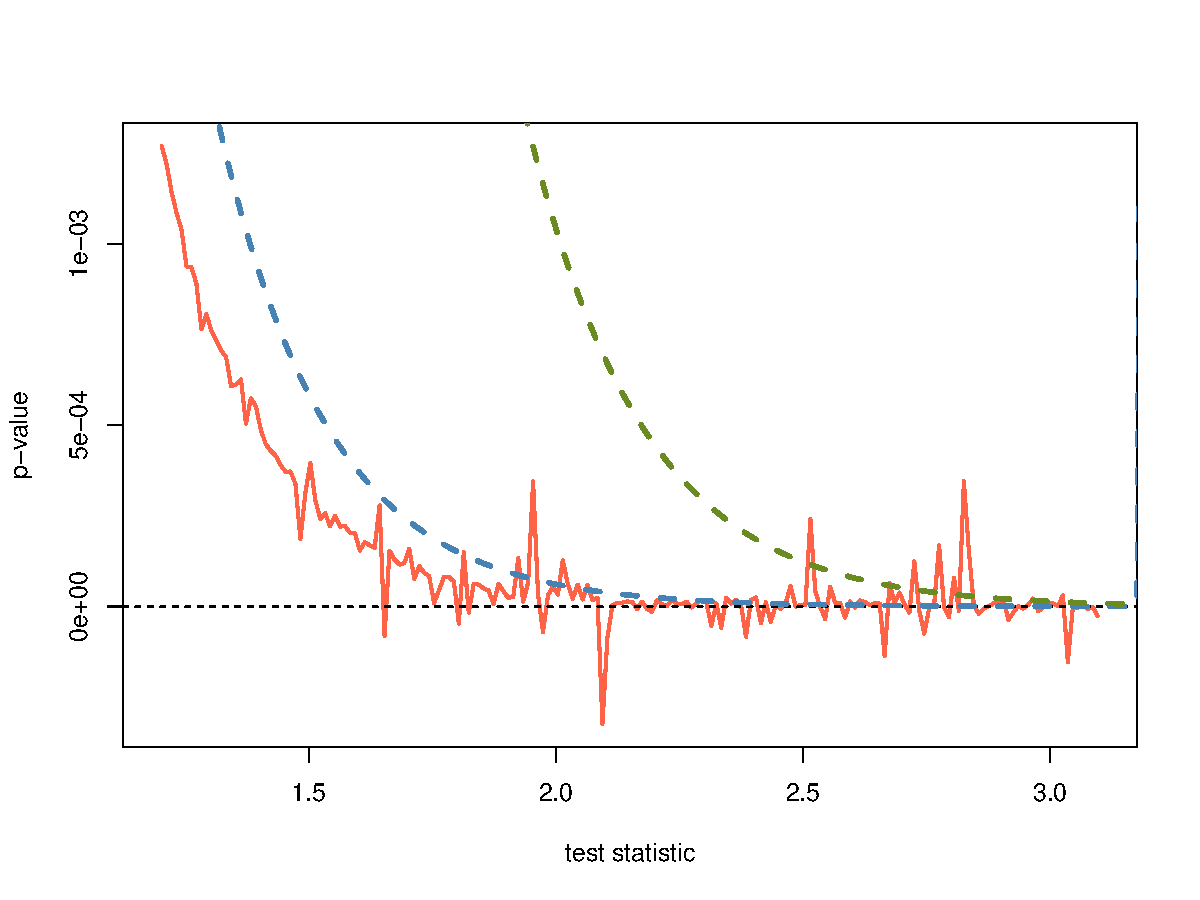
\includegraphics[scale=0.4]{fig1.pdf}
\end{center}
\caption{Plot of p-value for given test statistics using numerical integration
(pink) versus a conservative chi-squared bound (blue). }
\label{cvmissues}
\end{figure}


%%%%%%%%%%%%%%%%%%%%%%%%%%%%%%%%%%%%%%%%%%%%%%%%%%%%%%
\section{Kolmogorov-Smirnov and Cram\'{e}r-von Mises Tests in R}

Functions \code{ks.test()} and \code{cvm.test()} are provided for
convenience in packages \pkg{ks.test} and \pkg{cvm.test}, respectively.
Function \code{ks.test()} offers a revision of
R's Kolmogorov-Smirnov function \code{ks.test()} from base
package \pkg{stats}, while \code{cvm.test()} is a new
function for Cram\'{e}r-von Mises tests.
Both are available from the authors
or from R-Forge (\url{https://r-forge.r-project.org/R/?group_id=802});
they will be proposed for inclusion in \pkg{stats} in late 2010.

The revised \pkg{ks.test()} function supports one-sample tests for discrete
null distributions by allowing the second argument, \code{y}, to be
an empirical cumulative distribution function (an R function
with class \code{ecdf}) or an object of class \code{stepfun} specifying
a discrete distribution.  As in the original version of \code{ks.test()},
the presence of ties in the data (the first argument, \code{x}) generates a
warning unless \code{y} describes a discrete distribution.  When a discrete
distribution is specified, exact p-values are not available for 
two-sided alternative hypotheses, but the reported p-values will be
conservative.  For one-sided tests,
exact p-values are calculated using Conover's
method (when \code{exact = NULL} or \code{exact = TRUE})
if the sample size is less than or equal to 30; otherwise, asymptotic distributions
are used which are reliable in such cases (CITATION? Is this correct?).
When \code{exact = FALSE} the asymptotic distribution is used which is known
to be imprecise but conservative, even for small samples (CITATION).

*** Discussion of what we might have broken: cases where the user
provided a discrete distribution to the original ks.test() even though
it wasn't intended to be supported. ***

The function \pkg{cvm.test()} is similar to \pkg{ks.test()}.  Its first two
arguments specify the data and null distribution; the only extra option,
\code{type}, specifies the variant of the Cram\'{e}r-von Mises test:
\begin{itemize}
\item \code{x}: a numerical vector of data values.
\item \code{y}: an \code{ecdf} or step-function (\code{stepfun}) for specifying
the null model
\item \code{type}: the variant of the Cram\'{e}r-von Mises test; \code{W2}
is the default and most common method, \code{U2} is for cyclical data,
and \code{A2} is the Anderson-Darling alternative.
\end{itemize}
As with \code{ks.test()}, \code{cvm.test()} returns an object of class 
\code{htest}.

 
%%%%%%%%%%%%%%%%%%
\section{Examples}

Consider a toy example, with observed data of length 2 (specifically, the
values 0 and 1) and a hypothized null distribution that places equal
probability on the values 0 and 1.  With the current \code{ks.test()} function
in R (which, admittedly, doesn't claim to handle discrete distributions),
the reported p-value, 0.5, is clearly incorrect:
\begin{Schunk}
\begin{Sinput}
> stats::ks.test(c(0, 1), ecdf(c(0, 1)))
\end{Sinput}
\begin{Soutput}
	One-sample Kolmogorov-Smirnov test

data:  c(0, 1) 
D = 0.5, p-value = 0.5
alternative hypothesis: two-sided 
\end{Soutput}
\end{Schunk}
Instead, the value of $D$ given in equation (1)
should be 0 and the associated p-value should be 1.  Our revision of \code{ks.test()}
fixes this problem when the user provides a discrete distribution:
\begin{Schunk} 
\begin{Sinput}
> ks.test(c(0, 1), ecdf(c(0, 1)))
\end{Sinput}
\begin{Soutput}
	One-sample Kolmogorov-Smirnov test

data:  c(0, 1) 
D = 0, p-value = 1
alternative hypothesis: two-sided 
\end{Soutput}
\end{Schunk}

Next, we simulate a sample of 25 from the discrete uniform distribution on
the integers $\{1, 2, \ldots, 10\}$ and show several variants of the
new \code{ks.test()} implementation.  The first is the default two-sided test,
where the reported p-value is a conservative upper bound for the actual
p-value.  In this case, the approximation may not be that tight, but this is
irrelevant for such large p-values (for more interesting p-values, the
upper bound is very close to the true p-value).
\begin{Schunk}
\begin{Sinput}
> library(ks.test)
> set.seed(1)
> x <- sample(1:10, 25, replace = TRUE)
> x
\end{Sinput}
\begin{Soutput}
 [1]  3  4  6 10  3  9 10  7  7  1  3  2  7
[14]  4  8  5  8 10  4  8 10  3  7  2  3
\end{Soutput}
\begin{Sinput}
> ks.test(x, ecdf(1:10))
\end{Sinput}
\begin{Soutput}
	One-sample Kolmogorov-Smirnov test

data:  x 
D = 0.08, p-value = 1
alternative hypothesis: two-sided 
\end{Soutput}
\end{Schunk}
Next, we conduct the default one-sided test, where Conover's method
provides the exact p-value (up to the numerical precision of the
implementation):
\begin{Schunk}
\begin{Sinput}
> ks.test(x, ecdf(1:10), alternative = "g")
\end{Sinput}
\begin{Soutput}
	One-sample Kolmogorov-Smirnov test

data:  x 
D^+ = 0.04, p-value = 0.7731
alternative hypothesis:
the CDF of x lies above the null hypothesis 
\end{Soutput}
\end{Schunk}
In contrast, the option \code{exact=FALSE} results in the
p-value obtained by applying the classical Kolmogorov-Smirnov
test, resulting in a conservative p-value:
\begin{Schunk}
\begin{Sinput}
> ks.test(x, ecdf(1:10), alternative = "g", 
+         exact = FALSE)
\end{Sinput}
\begin{Soutput}
	One-sample Kolmogorov-Smirnov test

data:  x 
D^+ = 0.04, p-value = 0.9231
alternative hypothesis:
the CDF of x lies above the null hypothesis 
\end{Soutput}
\end{Schunk}

JAY: reconsider simulation.  Not really needed, if we have citations for
the conservatism points, etc...?  The code for this is in the JSS folder.
if we want to revisit it.

Finally, we employ two of the Cram\'{e}r-von Mises tests.  Taylor, are these
your ``cynical example'' that you commented on, or did you have something
in addition to these?  What should be discussed here?

\begin{Schunk}
\begin{Sinput}
> library(cvm.test)
> cvm.test(x, ecdf(1:10))
\end{Sinput}
\begin{Soutput}
	Cramer-von Mises - W2

data:  x 
W2 = 0.057, p-value = 0.8114
alternative hypothesis: Two.sided 
\end{Soutput}
\begin{Sinput}
> cvm.test(x, ecdf(1:10), type = "A2")
\end{Sinput}
\begin{Soutput}
	Cramer-von Mises - A2

data:  x 
A2 = 0.3969, p-value = 0.75
alternative hypothesis: Two.sided 
\end{Soutput}
\end{Schunk}

TAYLOR: good cyclical example, relating to new material about to go into
earlier section.


\section{Discussion}

The chi-squared test is a popular alternative to the methods presented here for doing goodness-of-fit tests for discrete data.
It differs by using no information about the geometry of the distribution, instead relying only the difference between the 
number of data points observed at each value and the expected number of data points that should be observed at each point. 
This generally has the effect of having a greater power towards alternatives with sharply different densities on a few points,
at the expense of losing power for alternatives with slight deviations over all of the points. Also, the non-parametric tests
have an advantage of being useful when the sample size is lower compared to the support of the distribution. The chi-squared
test is generally not used unless there are at least five data points in each element of the support. On the other hand,
chi-squared can be used in situations when there is not a numerical interpretation of the observation space 
(e.g. a set of ethnicities).
For a more complete comparison of the two tests' power see \cite{slakter65}.

The computational capabilities of modern computers provide an alternative to using a complex formula to
calculate the p-value for a test statistic. By drawing random samples from the null distribution, in many
cases the p-values for a given statistic can be calculated accurately in a relatively short time span.
This can be quite useful in some cases, but using the exact formulas from our methodology has several
distinct advantages. First of all, if the function is called many times (say, within another simulation
study), the computational benefits of using a formula can quickly become substantial. There is also a greater need
for supervision in a simulation study, with the exact number of runs needed to reach convergence (or other 
similar threshold). Additionally, while
simulations are generally a well received accepted method, it is often important in applied data analysis
to be sure that the calculated $p$-values are not the result of a numerical oddity in a particular
run of a simulation. 

In the end, for methods such as those presented in this paper where it is possible,
there are enough positives to suggest that we attempt to implement exact $p$-value calculations. This does lead
to an interesting direction for future research in non-parametric goodness of fit tests: the methods presented
here were historically chosen because they could be shown to have fixed null distributions which could easily
calculated in an era without fast computers for carrying out permutation tests. It is quite possible that
variants without the property, which could be easily used today, have greater power to certain alternative 
distributions.

%Possibly go into a brief discussion of classes and class inheritance in R. The use of `htest' in our functions; benefits and issues with using it. Particularly troublesome in ks.test where we have a range of p-values.  More precisely, explain that we
%could provide upper and lower bounds for the p-value but are limited by class
%\code{htest}.

In the continuous setting, both the Kolmogorov-Smirnov and the Cram\'{e}r-von Mises tests have two sample analogues. Here data are
observed from two processes, and the hypothesis tested is whether they came from the same (but unspecified) distribution. There
does not exist an analogous theory for discrete distributions. This comes from the fact that the discrete null distributions
of the test statistics depend on the exact null distribution; therefore the two sample case would surely have to depend
on the exact distributions used as well, which are generally not even stated in the two-sample case. 

While we have implemented the two most popular variants of goodness-of-fit tests, there are 
several more exotic varieties to be found. For further generalizations of tests see the extended study done in \cite{dewev1973}.


%\bibliography{example}

\bibliography{paper}

\address{Taylor B. Arnold \\
Yale University\\
24 Hillhouse Ave. \\
New Haven, CT 06511
USA\\
}
\email{taylor.arnold@yale.edu}

\address{John W. Emerson \\
Yale University\\
24 Hillhouse Ave. \\
New Haven, CT 06511
USA\\
}
\email{john.emerson@yale.edu}

